\section{Experimentation} 
\label{sec:Experimentation}


The experiments were carried out on a computer with an Intel Core i7-3930K CPU 3,20 GHz processor, 64 GB of memory and running under Windows 10 Pro.
All algorithms were implemented in Java (openjdk-17) in an internal CP solver.

The results relate to the solving of four problems, 
the traveling salesman problem (TSP)~\cite{Isoart:Thetravelingsalesmanprobleminconstraintprogramming}, the StockingCost problem~\cite{Houndji:dataset_item}, the flexible job shop scheduling problem (FJSSP)~\cite{Pelleau:dataFJSSP,Weise:jsspInstancesAndResults} and a problem of assigning child to activities (CHILD)~\cite{Varone:dataCHILD}. The TSP data are the instances (77) of the TSPLIB~\cite{Reinelt:TSPLIB} having less than 1,500 cities. Some of them involve more than a million of edges. 
The StockingCost data are those used in a Houndji's paper~\cite{Houndji:dataset_item}, this is random data distributed define as 
100 instances with 500 periods. Precisely, 
the StockingCost instances have 500 variables and 500 values. 
The FJSSP data come from two different sources, given 
by Pelleau~\cite{Pelleau:dataFJSSP} and Weise~\cite{Weise:jsspInstancesAndResults}. There are 370 instances with between 5 and 20 variables linked to a few values (between 5 and 10), and most instances have between 50 and 300 arcs. 
The CHILD instance contains only real-life data from~\cite{Varone:dataCHILD}. There are 623 children and 317 activities. Each child must be assigned to one activity. One activity can be associated with multiple children.

For each instance of each problem, we measure the information relating to the establishment of the arc consistency of the costgcc constraint at the root of the search tree. The mean of the results for each data set are reported in the tables.

The $H$ value of the TSP instances comes from the heuristic of Lin-Kernighan~\cite{Lin:HeuristicTSP}. Most of the time, this value is the optimal value. For the instances 
StockingCost, FJSSP and CHILD the regular $H$ is the smallest value such that there exists at least one solution and the big $H$ is twice as large as the regular $H$.

It is important to pay close attention to the relationship between the value of $H$ and the value of the minimum-cost flow. Indeed, the costgcc constraint sometimes represents a lower bound of the optimal solution, and this lower bound can be more or less distant from the optimal solution. 
So if $H$ is the value of the optimal solution, then the min-cost flow may well have a much lower value.  This is particularly true for the TSP problem.

Shortest paths are computed by using Dijkstra's algorithm and strongly connected components are computed by using Tarjan's algorithm.

The following abbreviations are used for the landmark selection methods: C for the center selection, O for the outline selection, C \& O for the combination between center and outline, Deg for the selection based on the maximum degree and R for the random selection. In addition, line 5+ contains the minimum values for a number of landmarks ranging from 5 to 10.

\pagebreak

\subsection{Results Tables}

\begin{table}[h!]
    \centering
    \resizebox{0.6\columnwidth}{!}{
    \begin{tabular}{| c | c || c | c | c | c | c | c |}
         \hline
         & Régin & \multirow{2}{1.3cm}{Landmark Number} & C & O & C \& O & Deg & R \\
          & & &   &   &   &   &   \\
         \hline
         \hline
         \multirow{5}{2.1cm}{TSP ($\le$ 100 cities)} 
            & \multirow{4}{0.8cm}{57.6}
                & 1 & 31.7 & 36.3 & 36.2 & \textbf{27.7} & \textbf{27.7} \\
                & & 2 & 35.3 & 39.9 & 39.8 & 32.5 & 29.5 \\
                & & 3 & 38 & 42.7 & 42.5 & 32.5 & 28.5 \\
                & & 4 & 41.6 & 46.3 & 46.1 & 32 & 30.1 \\
                & & 5+ & 44.8 & 50 & 50.2 & 32 & 32.2 \\
         \hline
         \multirow{5}{2.1cm}{TSP ($>$ 100 \& $<$ 250 cities)}
            & \multirow{4}{0.8cm}{163.3}
               & 1 & 42.2 & 45 & 47.9 & \textbf{40.5} & \textbf{40.5} \\
               & & 2 & 44.4 & 47.4 & 46.3 & 41.6 & 41.6 \\
               & & 3 & 46 & 49.3 & 48.2 & 41.2 & 41.2 \\
               & & 4 & 48.6 & 51.9 & 50.8 & 42.3 & 42.3 \\
               & & 5+ & 50.2 & 54.1 & 52.2 & 43.1 & 43.3 \\
         \hline
         \multirow{5}{2.1cm}{TSP ($\ge$ 250 cities)}
           & \multirow{4}{0.8cm}{662.7}
               & 1 & 18.1 & 19.8 & 19.8 & 17.8 & 17.8 \\
               & & 2 & 18.5 & 21.4 & 21.4 & 18.1 & 18.1 \\
               & & 3 & 18.5 & 21 & 19.3 & \textbf{16.3} & \textbf{16.2} \\
               & & 4 & 18.8 & 21.6 & 19.9 & 16.4 & \textbf{16.3} \\
               & & 5+ & 19 & 21.8 & 20.1 & 16.7 & 16.4 \\
         \hline
         \multirow{5}{2.1cm}{StockingCost (Regular H)} 
           & \multirow{4}{0.8cm}{\textbf{493.3}}
               & 1 & 496.9 & 497.3 & 496.9 & 495.3 & 495.3 \\
               & & 2 & 500.8 & 501.2 & 500.8 & 497.3 & 497.2 \\
               & & 3 & 504.7 & 505.1 & 504.7 & 499.2 & 499.1 \\
               & & 4 & 508.6 & 509 & 508.6 & 501.2 & 501 \\
               & & 5+ & 512.5 & 512.9 & 512.6 & 503.2 & 503 \\
         \hline
         \multirow{5}{2.1cm}{StockingCost (Big H)} 
           & \multirow{4}{0.8cm}{493.3}
               & 1 & 4 & 4 & 4 & \textbf{2} & \textbf{2} \\
               & & 2 & 4 & 4 & 4 & \textbf{2} & \textbf{2} \\
               & & 3 & 4 & 4 & 4 & \textbf{2} & \textbf{2} \\
               & & 4 & 4 & 4 & 4 & \textbf{2} & \textbf{2} \\
               & & 5+ & 4 & 4 & 4 & \textbf{2} & \textbf{2} \\
         \hline
         \multirow{5}{2.1cm}{FJSSP (Regular H)} 
           & \multirow{4}{0.8cm}{10.4}
               & 1 & 8.3 & 5.1 & 4.8 & \textbf{2} & 6.3 \\
               & & 2 & 8.3 & 5.1 & 4.8 & \textbf{2} & 5.3 \\
               & & 3 & 8.3 & 5.1 & 4.8 & \textbf{2} & 4.6 \\
               & & 4 & 8.3 & 5.1 & 4.8 & \textbf{2} & 4 \\
               & & 5+ & 8.3 & 5.1 & 4.8 & \textbf{2} & 4 \\
         \hline
         \multirow{5}{2.1cm}{FJSSP (Big H)} 
           & \multirow{4}{0.8cm}{10.4}
               & 1 & 4.5 & 4.3 & 4.3 & \textbf{2} & 3.2 \\
               & & 2 & 4.5 & 4.3 & 4.3 & \textbf{2} & 2.8 \\
               & & 3 & 4.5 & 4.3 & 4.3 & \textbf{2} & 2.6 \\
               & & 4 & 2.9 & 4.3 & 4.3 & \textbf{2} & 2.4 \\
               & & 5+ & 2.9 & 4.3 & 4.3 & \textbf{2} & 2.4 \\
         \hline
         \multirow{5}{2.1cm}{CHILD (Regular H)} 
           & \multirow{4}{0.8cm}{\textbf{108}}
               & 1 & 112 & 112 & 112 & 109 & 110 \\
               & & 2 & 116 & 116 & 116 & 111 & 112 \\
               & & 3 & 120 & 120 & 120 & 113 & 114 \\
               & & 4 & 124 & 124 & 124 & 115 & 116 \\
               & & 5+ & 128 & 128 & 128 & 117 & 118 \\
         \hline
         \multirow{5}{2.1cm}{CHILD (Big H)} 
           & \multirow{4}{0.8cm}{108}
               & 1 & 4 & 4 & 4 & \textbf{2} & \textbf{2} \\
               & & 2 & 4 & 4 & 4 & \textbf{2} & \textbf{2} \\
               & & 3 & 4 & 4 & 4 & \textbf{2} & \textbf{2} \\
               & & 4 & 4 & 4 & 4 & \textbf{2} & \textbf{2} \\
               & & 5+ & 4 & 4 & 4 & \textbf{2} & \textbf{2} \\
         \hline
    \end{tabular}
    }
    \caption{Establishment of the arc consistency of a costgcc constraint: average number of computed shortest paths
    depending on the number of landmarks and the landmark selection method.}
    \label{tab:numberOfShortestPath}
\end{table}

\begin{table}[!ht]
    \centering
    \resizebox{0.7\columnwidth}{!}{
    \begin{tabular}{| c || c | c | c | c | c | c |}
         \hline
         & Régin & C & O & C \& O & Deg & R \\
         \hline
         \hline
         TSP ($\le$ 100 cities)
              & 35.8 & 19.7 & 24.4 & 24.3 & \textbf{8.3} & \textbf{8.2}  \\
               
         \hline
         TSP ($>$ 100 \& $<$ 250 cities) 
               & 131.1 & 16 & 19.7 & 18.6 & \textbf{10.1} & \textbf{10.1}  \\
               
         \hline
         TSP ($\ge$ 250 cities)
               & 649.8 & 5.9 & 8.6 & 6.9 & \textbf{3.4} & \textbf{3.3}  \\
               
         \hline
         StockingCost (Regular H)
                & \textbf{0} & 3.2 & 7.6 & 11.2 & 7.8 & 7.6 \\               
         \hline
         StockingCost (Big H)
                & 493.3 & 4 & 4 & 4 & \textbf{2} & \textbf{2} \\
               
         \hline
         FJSSP (Regular H)
                & \textbf{0} & 8.3 & 5.1 & 4.8 & 4 & 4 \\
               
         \hline
         FJSSP (Big H)
                & 10.1 & 2.9 & 4.3 & 4.3 & \textbf{2} & 2.4 \\
                
         \hline
         CHILD (Regular H)
               & \textbf{0} & 16 & 16 & 16 & 8 & 8 \\
               
         \hline
         CHILD (Big H)
                & 108 & 4 & 4 & 4 & \textbf{2} & \textbf{2} \\
                
         \hline
    \end{tabular}
    }
    \caption{Establishment of the arc consistency of a costgcc constraint: number of average shortest paths computed uselessly with 4 landmarks.}
    \label{tab:numberSPUseless}
\end{table}


\begin{table}[!ht]
    \centering
    \resizebox{0.7\columnwidth}{!}{
    \begin{tabular}{| c | c || c | c | c | c | c | c |}
         \hline
         & & Régin & C & O & C \& O & Deg & R \\
         \hline
         \hline
         \multirow{3}{2.1cm}{TSP ($\le$ 100 cities)} 
               & Mean & 7.3 & 5.9 & 6 & 6.6 & 5.7 & \textbf{4.5} \\
               & Median & 3.4 & 3.6 & 4.4 & 4.1 & 3.6 & \textbf{3.3} \\
               & Ratio & & 1.2 & 1.2 & 1.1 & 1.3 & \textbf{1.6} \\
         \hline
         \multirow{3}{2.1cm}{TSP ($>$ 100 \& $<$ 250 cities)} 
               & Mean & 76.6 & \textbf{29.8} & 30.6 & 30.2 & \textbf{28.6} & 31.1 \\
               & Median & 51.2 & \textbf{14.3} & 16 & 17 & 15.4 & \textbf{14.3} \\
               & Ratio & & \textbf{2.6} & 2.5 & 2.5 & \textbf{2.7} & 2.5 \\
         \hline
         \multirow{3}{2.1cm}{TSP ($\ge$ 250 cities)}
               & Mean & 12124.9 & 278.9 & 275.2 & 275.4 & \textbf{213} & 265 \\
               & Median & 2310.2 & 126.8 & 117.7 & 90.6 & 89.1 & \textbf{85.9} \\
               & Ratio & & 43.5 & 44.1 & 44 & \textbf{56.9} & 45.8 \\
         \hline
         \multirow{3}{2.1cm}{StockingCost (Regular H)} 
               & Mean & 603.83 & \textbf{511.8} & 617.9 & 626.2 & 580.3 & 639.4 \\
               & Median & 585.7 & 553.3 & 186.9 & 186.4 & 248 & \textbf{166.4} \\
               & Ratio & & \textbf{1.2} & 1 & 1 & 1 & 0.9 \\
         \hline
         \multirow{3}{2.1cm}{StockingCost (Big H)} 
               & Mean & 534.76 & 34.1 & 32.4 & \textbf{31.6} & 33.2 & 32.6 \\
               & Median & 519.1 & 33.8 & 32.4 & 31.9 & 32.8 & \textbf{30.1} \\
               & Ratio & & 15.7 & 16.5 & \textbf{16.9} & 16 & 16.4 \\
         \hline
         \multirow{3}{2.1cm}{FJSSP (Regular H)} 
               & Mean & 0.4 & 0.5 & \textbf{0.3} & 0.4 & 0.4 & 0.5 \\
               & Median & \textbf{0.1} & 0.3 & 0.2 & 0.3 & 0.2 & 0.3 \\
               & Ratio & & 0.8 & \textbf{1.7} & 0.75 & 1 & 0.8 \\
         \hline
         \multirow{3}{2.1cm}{FJSSP (Big H)} 
               & Mean & 0.4 & 0.4 & \textbf{0.3} & \textbf{0.3} & \textbf{0.3} & \textbf{0.3} \\
               & Median & \textbf{0.1} & 0.2 & 0.2 & 0.2 & 0.2 & 0.2 \\
               & Ratio & & 1 & \textbf{1.3} & \textbf{1.3} & \textbf{1.3} & \textbf{1.3} \\
         \hline
         \multirow{2}{2.1cm}{CHILD (Regular H)} 
               & Time & 65.1 & 69.2 & \textbf{54.4} & 67.6 & 75.9 & 65.4 \\
               & Ratio & & 0.9 & \textbf{1.2} & 1 & 0.8 & 1 \\
         \hline
         \multirow{2}{2.1cm}{CHILD (Big H)} 
               & Time & 58.2 & 7 & 6.5 & 7.3 & \textbf{6} & \textbf{6} \\
               & Ratio & & 8.3 & 9 & 8 & \textbf{9.7} & \textbf{9.7} \\
         \hline
    \end{tabular}
    }
    \caption{Establishment of the arc consistency of a costgcc constraint: computation times (in ms) and ratio. Experimentation with 4 landmarks.}
    \label{tab:timeWithMagic}
\end{table}

We consider a shortest path calculation to be the calculation of the shortest paths from one node to all the others. 

The number of shortest paths calculated is an important parameter for distinguishing between algorithms. 
Some shortest path computations cannot be avoided, particularly those required to detect inconsistent values. 
However, some shortest path computations are useless, as they do not allow us to establish the inconsistency of any value. Precisely, if the shortest path computation from $b$ In Corollary~\ref{acpte} does not lead to any deletion of values then this path computation is useless. 

Table~\ref{tab:numberOfShortestPath} compares the number of shortest path computations performed by Régin's algorithm and by our approach as a function of the number of landmarks allowed in. The number of shortest paths required to compute landmarks are included.

Table~\ref{tab:numberSPUseless} shows the average number of useless shortest path computations for each dataset. We consider that shortest path computations for landmarks are always useless, so they are always included. That is why there are never $0$ computations with landmarks. 

Table~\ref{tab:timeWithMagic} gives the time required by each method.

\subsection{Results Analysis}

Table~\ref{tab:numberOfShortestPath} shows that our approach generally computes significantly fewer shortest paths than Régin's algorithm for all landmarks selection methods. For the TSP instances, we compute on average between 2 and 47 times fewer shortest paths than Régin's algorithm. The difference is significant for all instances except for the StockingCost instances with Regular H.
It should be noted that our approach is always better or equivalent and allows us to detect quickly whether the constraint is arc consistent in certain cases.

In the best case, our approach does not compute any shortest paths other than those required to determine landmarks. Our approach can compute more shortest paths only when there is no inconsistent arc and the extra computation is due to the landmarks.
The number of useless path computations is also reduced by our method (See Table~\ref{tab:numberSPUseless}).

For computation times, we find the same kind of results as before (See Table~\ref{tab:timeWithMagic}). The gain average factors evolve between $1$ and $57$. 

\subsubsection{Landmark Number and Selection Method}

We can see that the results do not change much as a function of the number of landmarks.
The major part of problems have best or equivalent results with 4 landmarks, but the difference is minimal. When it is not mentioned $4$ landmarks are used. 

Two methods of landmark selection appear to be more effective in practice: the method based on maximum node degrees and the random node selection method. As there is little difference between these two methods, and the former is more robust than the latter, we recommend defining landmarks based on maximum degree nodes. 

\subsubsection{Impact of the practical improvement of Section 5}

Thanks to this practical improvement all the authorized landmarks are not systematically used. This is clearly seen for StockingCost and CHILD instances with big $H$. The computation of a single landmark is sufficient to guarantee that all the values are consistent.

\subsubsection{StockingCost, FJSSP and CHILD problems}

For the StockingCost, FJSSP and CHILD problems, the results strongly depends on the value of $H$.

For the Regular $H$ value the results are similar to those of Régin's algorithm. In these problems, Regular $H$ is close to the optimal value of the min cost flow of the underlined costgcc.
Thus, there is less margin and therefore more inconsistent values.
FJSSP instances are also small and do not allow us to highlight the usefulness of landmarks. Indeed, in a small instance, computing a landmark gives us access to less information than in a large instance. In addition, for practical use, it is more interesting to save time on large instances since they take longer to resolve than on small instances which are already quick to resolve.

For a Big $H$ value the landmark method clearly outperforms Régin's algorithm.

\begin{figure}[ht!]
    \begin{subfigure}[t]{0.33\columnwidth}
    \resizebox{1.1\columnwidth}{!}{
        \centering
        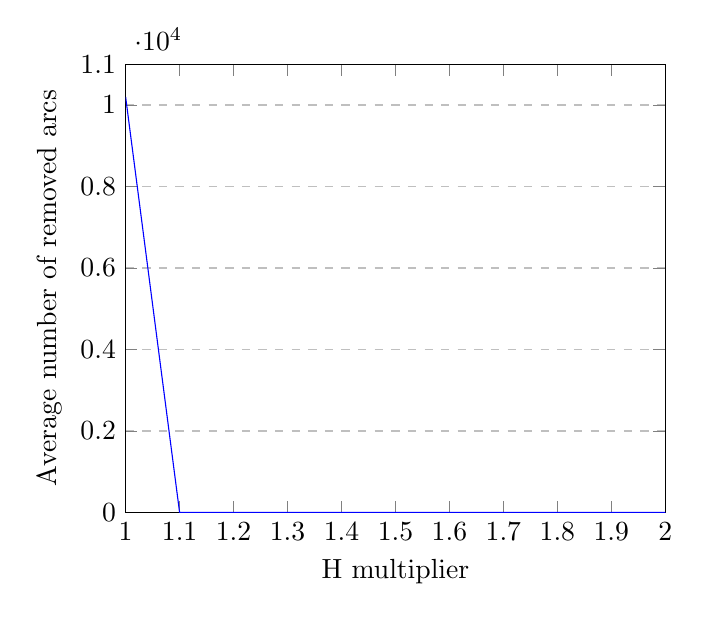
\begin{tikzpicture}
    \begin{axis}[
        xlabel={H multiplier},
        ylabel={Average number of removed arcs},
        xmin=1, xmax=2,
        ymin=0, ymax=11000,
        xtick={1, 1.1, 1.2, 1.3, 1.4, 1.5, 1.6, 1.7, 1.8, 1.9, 2},
        ytick={0, 2000, 4000, 6000, 8000, 10000, 11000},
        legend pos=north west,
        ymajorgrids=true,
        grid style=dashed,
    ]



    \addplot[
        color=blue,
        ]
        coordinates {
    (1, 10195.0) (1.1, 0.0) (1.2, 0.0) (1.3, 0.0) (1.4, 0.0) (1.5, 0.0) (1.6, 0.0) (1.7, 0.0) (1.8, 0.0) (1.9, 0.0) (2, 0.0)     };
        
    \end{axis}
    \end{tikzpicture}
    }
        \subcaption{CHILD}
    \end{subfigure}
    \quad
    \begin{subfigure}[t]{0.3\columnwidth}
    \resizebox{1.1\columnwidth}{!}{
        \centering
        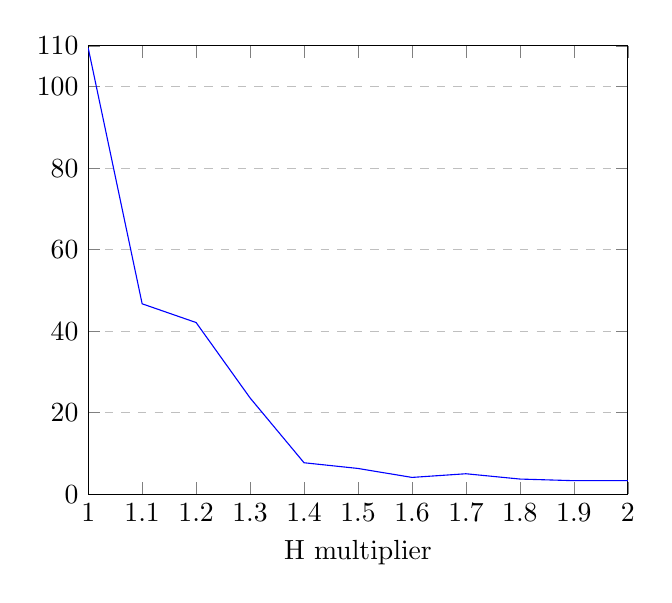
\begin{tikzpicture}
    \begin{axis}[
        xlabel={H multiplier},
        xmin=1, xmax=2,
        ymin=0, ymax=110,
        xtick={1, 1.1, 1.2, 1.3, 1.4, 1.5, 1.6, 1.7, 1.8, 1.9, 2},
        ytick={0, 20, 40, 60, 80, 100, 110},
        legend pos=north west,
        ymajorgrids=true,
        grid style=dashed,
    ]



    \addplot[
        color=blue,
        ]
        coordinates {
    (1, 109.5) (1.1, 46.7) (1.2, 42.1) (1.3, 23.6) (1.4, 7.7) (1.5, 6.3) (1.6, 4.1) (1.7, 5) (1.8, 3.7) (1.9, 3.3) (2, 3.3)      };
        
    \end{axis}
    \end{tikzpicture}
    }
        \subcaption{FJSSP}
    \end{subfigure}
    \quad
    \begin{subfigure}[t]{0.3\columnwidth}
    \resizebox{1.1\columnwidth}{!}{
        \centering
        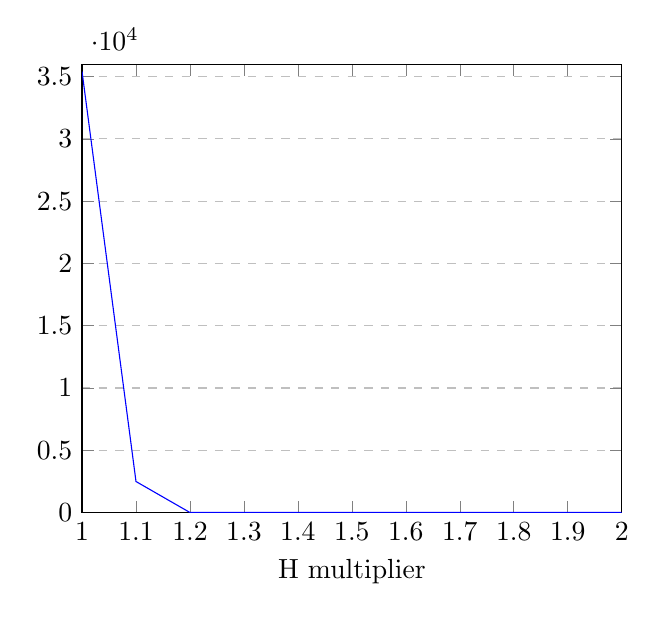
\begin{tikzpicture}
    \begin{axis}[
        xlabel={H multiplier},
        xmin=1, xmax=2,
        ymin=0, ymax=36000,
        xtick={1, 1.1, 1.2, 1.3, 1.4, 1.5, 1.6, 1.7, 1.8, 1.9, 2},
        ytick={0, 5000, 10000, 15000, 20000, 25000, 30000, 35000},
        legend pos=north west,
        ymajorgrids=true,
        grid style=dashed,
    ]



    \addplot[
        color=blue,
        ]
        coordinates {
    (1, 35410.1) (1.1, 2489.1) (1.2, 0.0) (1.3, 0.0) (1.4, 0.0) (1.5, 0.0) (1.6, 0.0) (1.7, 0.0) (1.8, 0.0) (1.9, 0.0) (2, 0.0)       };        
    \end{axis}
    \end{tikzpicture}
    }
        \subcaption{StockingCost}
        \end{subfigure}
    \caption{Evolution of the average number of removed arcs for the CHILD, FJSSP and StockingCost instances in function of the multiplier of $H$.}
    \label{fig:averageNumberOfRemovedArcInFunctionOfH}
\end{figure}

\begin{figure}[ht!]
    \begin{subfigure}[t]{0.33\columnwidth}
    \resizebox{1.1\columnwidth}{!}{
         \centering
        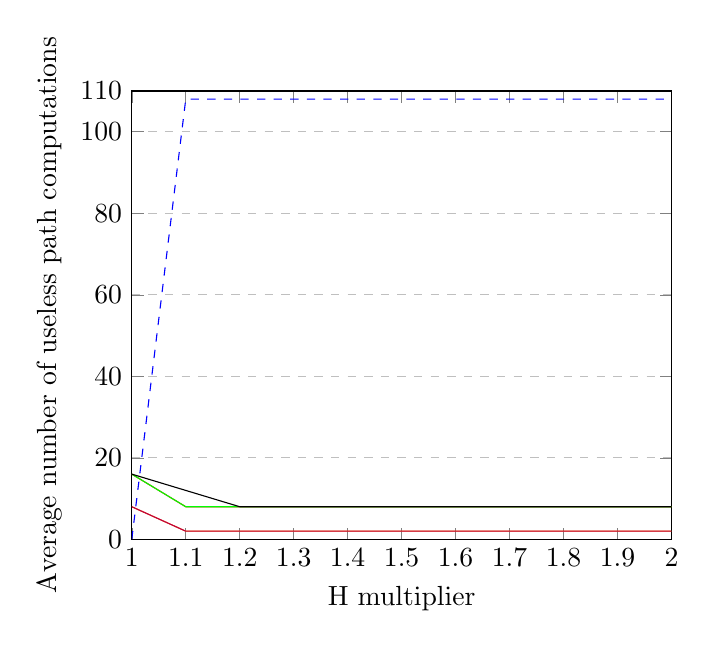
\begin{tikzpicture}
    \begin{axis}[
        xlabel={H multiplier},
        ylabel={Average number of useless path computations},
        xmin=1, xmax=2,
        ymin=0, ymax=110,
        xtick={1, 1.1, 1.2, 1.3, 1.4, 1.5, 1.6, 1.7, 1.8, 1.9, 2},
        ytick={0, 20, 40, 60, 80, 100, 110},
        legend style={xshift=2cm},
        legend pos=north west,
        ymajorgrids=true,
        grid style=dashed,
    ]



    \addplot[
        dashed,
        color=blue,
        ]
        coordinates {
    (1, 0.0) (1.1, 108.0) (1.2, 108.0) (1.3, 108.0) (1.4, 108.0) (1.5, 108.0) (1.6, 108.0) (1.7, 108.0) (1.8, 108.0) (1.9, 108.0) (2, 108.0)        };



    \addplot[
        color=red,
        ]
        coordinates {
    (1, 16.0) (1.1, 8.0) (1.2, 8.0) (1.3, 8.0) (1.4, 8.0) (1.5, 8.0) (1.6, 8.0) (1.7, 8.0) (1.8, 8.0) (1.9, 8.0) (2, 8.0) };

    \addplot[
        color=green,
        ]
        coordinates { 
    (1, 16.0) (1.1, 8.0) (1.2, 8.0) (1.3, 8.0) (1.4, 8.0) (1.5, 8.0) (1.6, 8.0) (1.7, 8.0) (1.8, 8.0) (1.9, 8.0) (2, 8.0)     };

    \addplot[
        ]
        coordinates {
    (1, 16.0) (1.1, 12.0) (1.2, 8.0) (1.3, 8.0) (1.4, 8.0) (1.5, 8.0) (1.6, 8.0) (1.7, 8.0) (1.8, 8.0) (1.9, 8.0) (2, 8.0) 
    };

    \addplot[
        color=orange,
        ]
        coordinates {
    (1, 8.0) (1.1, 2.0) (1.2, 2.0) (1.3, 2.0) (1.4, 2.0) (1.5, 2.0) (1.6, 2.0) (1.7, 2.0) (1.8, 2.0) (1.9, 2.0) (2, 2.0) };
    
    \addplot[
        color=purple,
        ]
        coordinates {
    (1, 8.0) (1.1, 2.0) (1.2, 2.0) (1.3, 2.0) (1.4, 2.0) (1.5, 2.0) (1.6, 2.0) (1.7, 2.0) (1.8, 2.0) (1.9, 2.0) (2, 2.0) 
    };
            
    \end{axis}
    \end{tikzpicture}
    }
        \subcaption{CHILD}
    \end{subfigure}
    \quad
    \begin{subfigure}[t]{0.3\columnwidth}
    \resizebox{1.1\columnwidth}{!}{
        \centering
        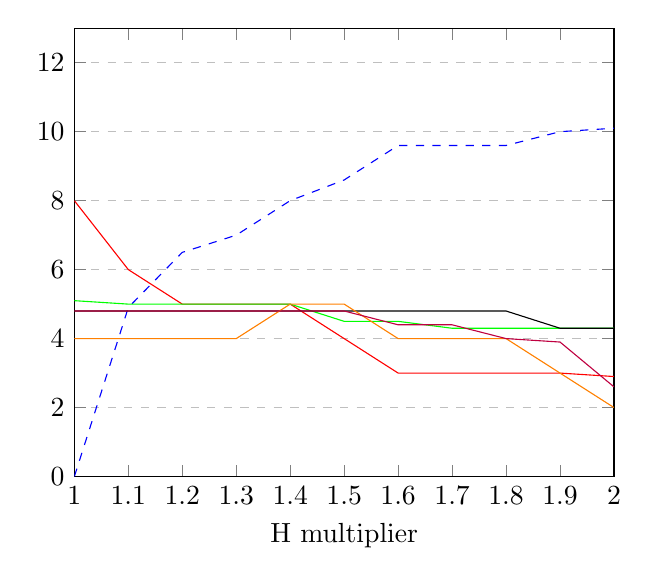
\begin{tikzpicture}
    \begin{axis}[
        xlabel={H multiplier},
        xmin=1, xmax=2,
        ymin=0, ymax=13,
        xtick={1, 1.1, 1.2, 1.3, 1.4, 1.5, 1.6, 1.7, 1.8, 1.9, 2},
        ytick={0, 2, 4, 6, 8, 10, 12},
        legend style={xshift=1.2cm},
        legend pos=north west,
        ymajorgrids=true,
        grid style=dashed,
    ]

    \addplot[
        color=blue,
        dashed,
        ]
        coordinates {
    (1, 0) (1.1, 4.9) (1.2, 6.5) (1.3, 7) (1.4, 8) (1.5, 8.6) (1.6, 9.6) (1.7, 9.6) (1.8, 9.6) (1.9, 10) (2, 10.1)       };

    \addplot[
        color=red,
        ]
        coordinates { 
    (1, 8) (1.1, 6) (1.2, 5) (1.3, 5) (1.4, 5) (1.5, 4) (1.6, 3) (1.7, 3) (1.8, 3) (1.9, 3) (2, 2.9) 
            };



            \addplot[
        color=green,
        ]
        coordinates { 
    (1, 5.1) (1.1,5) (1.2, 5) (1.3, 5) (1.4, 5) (1.5, 4.5) (1.6, 4.5) (1.7, 4.3) (1.8, 4.3) (1.9, 4.3) (2, 4.3) 
            };

            \addplot[
        ]
        coordinates { 
    (1, 4.8) (1.1, 4.8) (1.2, 4.8) (1.3, 4.8) (1.4, 4.8) (1.5, 4.8) (1.6, 4.8) (1.7, 4.8) (1.8, 4.8) (1.9, 4.3) (2, 4.3) 
            };
            
            \addplot[
        color=orange,
        ]
        coordinates {
    (1, 4) (1.1, 4) (1.2, 4) (1.3, 4) (1.4, 5) (1.5, 5) (1.6, 4) (1.7, 4) (1.8, 4) (1.9, 3) (2, 2) 
            };
            \addplot[
        color=purple,
        ]
        coordinates {
    (1, 4.8) (1.1, 4.8) (1.2, 4.8) (1.3, 4.8) (1.4, 4.8) (1.5, 4.8) (1.6, 4.4) (1.7, 4.4) (1.8, 4) (1.9, 3.9) (2, 2.6) 
            };
    \end{axis}
    \end{tikzpicture}
    }
        \subcaption{FJSSP}
    \end{subfigure}
    \quad
    \begin{subfigure}[t]{0.3\columnwidth}
    \resizebox{1.1\columnwidth}{!}{
        \centering
        \begin{tikzpicture}
    \begin{axis}[
        xlabel={H multiplier},
        xmin=1, xmax=2,
        ymin=0, ymax=500,
        xtick={1, 1.1, 1.2, 1.3, 1.4, 1.5, 1.6, 1.7, 1.8, 1.9, 2},
        ytick={0, 100, 200, 300, 400, 500},
        legend style={xshift=4cm},
        legend pos=north west,
        ymajorgrids=true,
        grid style=dashed,
    ]



    \addplot[
        dashed,
        color=blue,
        ]
        coordinates {
    (1, 0.0) (1.1, 479.3) (1.2, 493.2) (1.3, 493.2) (1.4, 493.2) (1.5, 493.2) (1.6, 493.2) (1.7, 493.2) (1.8, 493.2) (1.9, 493.2) (2, 493.2)        };



\addplot[
        color=red,
        ]
        coordinates {
    (1, 3.2) (1.1, 58.7) (1.2, 6.2) (1.3, 4.0) (1.4, 4.0) (1.5, 4.0) (1.6, 4.0) (1.7, 4.0) (1.8, 4.0) (1.9, 4.0) (2, 4.0) 
            };



            \addplot[
        color=green,
        ]
        coordinates {
    (1, 7.6) (1.1, 27.1) (1.2, 10.2) (1.3, 8.0) (1.4, 8.0) (1.5, 8.0) (1.6, 8.0) (1.7, 8.0) (1.8, 8.0) (1.9, 4.0) (2, 4.0) 
            };
                \addplot[
        ]
        coordinates {
    (1, 11.2) (1.1, 30.8) (1.2, 14.1) (1.3, 12.0) (1.4, 12.0) (1.5, 12.0) (1.6, 12.0) (1.7, 12.0) (1.8, 12.0) (1.9, 12.0) (2, 12.0) 
            };
    \addplot[
        color=orange,
        ]
        coordinates {
    (1, 7.8) (1.1, 8.3) (1.2, 2) (1.3, 2.0) (1.4, 2.0) (1.5, 2.0) (1.6, 2.0) (1.7, 2.0) (1.8, 2.0) (1.9, 2.0) (2, 2.0)
            };
            \addplot[
        color=purple,
        ]
        coordinates {
    (1, 7.6) (1.1, 3.3) (1.2, 2.0) (1.3, 2.0) (1.4, 2.0) (1.5, 2.0) (1.6, 2.0) (1.7, 2.0) (1.8, 2.0) (1.9, 2.0) (2, 2.0) 
            };
    
        \legend{$Régin$, $C$, $O$, $C \& O$, $Deg$, $R$}
        
    \end{axis}
    \end{tikzpicture}
    }
        \subcaption{StockingCost}
    \end{subfigure}
   \caption{Evolution of the average number of useless path computations for CHILD, FJSSP and StockingCost instances in function of the multiplier of $H$. The experimentation involves 4 landmarks.}
    \label{fig:averageNumberOfUselessArcInFunctionOfH}
\end{figure}

Figures~\ref{fig:averageNumberOfRemovedArcInFunctionOfH} and~\ref{fig:averageNumberOfUselessArcInFunctionOfH}  provide information on the relationship between H values and the number of useless path computations. The landmark approach performs very well as soon as the H value deviates a little from the optimal value, in other words, as soon as there is a little margin and therefore fewer inconsistent values. 

\subsubsection{TSP results}

\begin{figure}[h!]
    \centering

    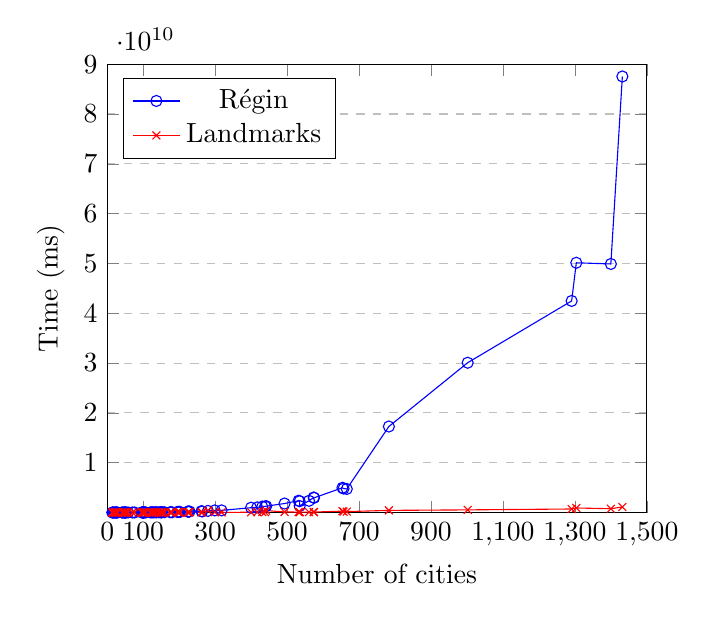
\begin{tikzpicture}
    \begin{axis}[
        xlabel={Number of cities},
        ylabel={Time (ms)},
        xmin=0, xmax=1500,
        ymin=0, ymax=90000000000,
        xtick={0, 100, 300, 500, 700, 900, 1100, 1300, 1500},
        ytick={10000000000,20000000000,30000000000,40000000000,50000000000, 60000000000, 70000000000, 80000000000, 90000000000},
        legend pos=north west,
        ymajorgrids=true,
        grid style=dashed,
    ]



    \addplot[
        color=blue,
        mark=o,
        ]
        coordinates {
    (14, 2220530) (16, 950000) (17, 860060) (21, 1116660) (24, 930200)
(24, 1197780) (26, 1486690) (29, 1601580) (42, 2264490)
(42, 2446820)
(48, 3118910)
(48, 3321220)
(48, 3078120)
(51, 3532080)
(52, 3958960)
(58, 4979160)
(70, 7667390)
(76, 8617660)
(96, 15848440)
(99, 17797560)
(100, 19894100)
(100, 16807600)
(100, 17191910)
(100, 15929530)
(100, 17003020)
(100, 16843160)
(101, 16479730)
(105, 18383100)
(107, 16535900)
(120, 27059660)
(124, 27427500)
(127, 30530280)
(130, 32565560)
(136, 38467470)
(137, 41165780)
(144, 37680510)
(150, 57056550)
(150, 50954690)
(150, 51381680)
(152, 49643640)
(159, 63188440)
(175, 64339780)
(180, 46947610)
(195, 110060270)
(198, 123414070)
(200, 121176790)
(200, 119243860)
(202, 113262300)
(225, 179283770)
(225, 182400100)
(226, 169735440)
(229, 202433870)
(262, 262275090)
(264, 214641530)
(280, 323887980)
(299, 419320610)
(318, 427294250)
(400, 964638060)
(417, 1030552820)
(431, 1183442850)
(439, 1229169640)
(442, 1274221000)
(493, 1801032960)
(532, 2370052470)
(535, 2266427160)
(535, 1297533110)
(561, 2353925570)
(574, 3013194430)
(575, 2942079820)
(654, 4967022570)
(657, 4805718030)
(666, 4732261640)
(783, 17263562430)
(1002, 30067701280)
(1291, 42474652160)
(1304, 50133037030)
(1400, 49894810930)
(1432, 87534613800)    };

\addplot[
        color=red,
        mark=x,
        ]
        coordinates {
        (14, 1227000)
(16, 1008700)
(17, 715060)
(21, 889450)
(24, 1101340)
(24, 1517620)
(26, 1705810)
(29, 2209810)
(42, 2610940)
(42, 2845160)
(48, 4204640)
(48, 3798670)
(48, 2919540)
(51, 4258940)
(52, 3812570)
(58, 2288940)
(70, 2172670)
(76, 9414520)
(96, 6725130)
(99, 20475770)
(100, 12123190)
(100, 4645240)
(100, 10093940)
(100, 3992920)
(100, 4676540)
(100, 6886930)
(101, 17637780)
(105, 2763470)
(107, 11454610)
(120, 16538910)
(124, 5575740)
(127, 6056090)
(130, 4051070)
(136, 41555070)
(137, 29285090)
(144, 5014980)
(150, 8717280)
(150, 9496670)
(150, 14327130)
(152, 9410730)
(159, 24582630)
(175, 6530950)
(180, 12352790)
(195, 99808970)
(198, 46652570)
(200, 10623980)
(200, 17352510)
(202, 30276280)
(225, 22996050)
(225, 58084130)
(226, 21101450)
(229, 30861490)
(262, 18296620)
(264, 34477980)
(280, 404324570)
(299, 59041250)
(318, 26636700)
(400, 47837750)
(417, 80016300)
(431, 88090960)
(439, 43850150)
(442, 386383150)
(493, 111820180)
(532, 79688030)
(535, 81409860)
(535, 73577830)
(561, 87960690)
(574, 87853650)
(575, 90140700)
(654, 272354330)
(657, 174685950)
(666, 180177550)
(783, 423349600)
(1002, 527210030)
(1291, 703587660)
(1304, 904640900)
(1400, 760029830)
(1432, 1111893000)
        };
        \legend{Régin, Landmarks}
        
    \end{axis}
    \end{tikzpicture}
    
    \caption{Evolution of the time in relation to the size of TSP instances. The landmarks are selected with the degree method and 4 landmarks. The blue plot with circles is the time of the Régin algorithm and the red with crosses is the time of the landmarks algorithm.}
    \label{fig:graphTime}
\end{figure}

The improvement brought about by our approach for instances from the TSP problem are strong. This is mainly due to the relationship between the $H$ value given by the TSP value and the underlying costgcc constraint. In the case of the TSP, the optimal value of the min cost flow is lower than $H$, because the costgcc constraint only models a part of the problem and in fact represents a real relaxation. So even with an optimal $H$ value for TSP, there is a margin for the costgcc constraint.

To better appreciate the performance of the landmarks, Figure~\ref{fig:graphTime} shows the evolution of time in milliseconds as a function of the size of the TSP dataset instances. The blue plot with circles shows the time taken by the Régin's algorithm, while the red plot with crosses shows the time taken by the algorithm using the maximum degrees and 4 landmarks. Clearly, the use of landmarks is drastically faster than the Régin's algorithm. The larger the instance, the more useful landmarks become.

Figure~\ref{fig:graphRatio} shows the evolution of the speed-up ratio (Régin time/Landmarks time) on the instances of the TSP dataset. The landmark selection algorithm is based on maximum degrees with 4 landmarks. We can also see in this graph that the more data there is, the higher the gain factor. As mentioned above, this can be explained by the fact that in a large structure, the landmarks contain a lot of information compared with a smaller structure. 
In these experiments, note that if we omit the assigned variables there is only one strongly connected component in the value network. Overall, we find that our algorithm significantly speeds up the previous approach, up to about 80 times faster for large problems. 


\begin{figure}[ht!]
    \centering
    \resizebox{0.6\columnwidth}{!}{

    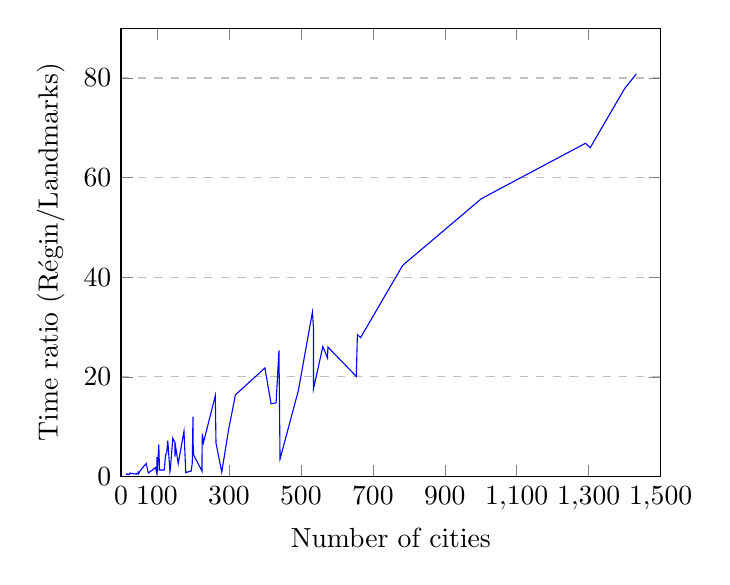
\begin{tikzpicture}
    \begin{axis}[
        xlabel={Number of cities},
        ylabel={Time ratio (Régin/Landmarks)},
        xmin=0, xmax=1500,
        ymin=0, ymax=90,
        xtick={0, 100, 300, 500, 700, 900, 1100, 1300, 1500},
        ytick={0,20,40,60,80, 100},
        legend pos=north west,
        ymajorgrids=true,
        grid style=dashed,
    ]



    \addplot[
        color=blue,
        ]
        coordinates {
    (14,0.6) (16,0.4) (17,0.5) (21,0.4) (24,0.4) (24,0.6) (26,0.7) (29,0.6) (42,0.5) (42,0.6) (48,0.5) (48,0.6) (48,0.9) (51,0.8) (52,1.0) (58,1.6) (70,2.6) (76,0.7) (96,1.8) (99,0.8) (100,1.4) (100,3.1) (100,1.6) (100,3.9) (100,3.3) (100,2.4) (101,0.9) (105,6.4) (107,1.3) (120,1.3) (124,4.4) (127,4.8) (130,7.2) (136,1.0) (137,1.4) (144,7.7) (150,6.8) (150,5.9) (150,4.0) (152,5.9) (159,2.6) (175,9.1) (180,0.8) (195,1.1) (198,2.7) (200,12.0) (200,7.0) (202,4.3) (225,1.1) (225,3.3) (226,8.6) (229,6.8) (262,16.2) (264,6.7) (280,0.9) (299,9.4) (318,16.4) (400,21.8) (417,14.6) (431,14.8) (439,25.3) (442,3.5) (493,17.3) (532,33.0) (535,29.7) (535,17.6) (561,26.1) (574,23.8) (575,26.0) (654,20.1) (657,28.5) (666,27.9) (783,42.4) (1002,55.8) (1291,66.9) (1304,66.0) (1400,77.9) (1432,80.8)    };
        
    \end{axis}
    \end{tikzpicture}
    }
    \caption{Evolution of the speedup ratio in relation to the size of TSP instances. The landmarks are selected with the degree method and 4 landmarks.}
    \label{fig:graphRatio}

\end{figure}






